\documentclass[10pt]{beamer}
\usetheme[
%%% option passed to the outer theme
%    progressstyle=fixedCircCnt,   % fixedCircCnt, movingCircCnt (moving is deault)
  ]{Feather}
  
% If you want to change the colors of the various elements in the theme, edit and uncomment the following lines

% Change the bar colors:
%\setbeamercolor{Feather}{fg=red!20,bg=red}

% Change the color of the structural elements:
%\setbeamercolor{structure}{fg=red}

% Change the frame title text color:
%\setbeamercolor{frametitle}{fg=blue}

% Change the normal text color background:
%\setbeamercolor{normal text}{fg=black,bg=gray!10}

%-------------------------------------------------------
% INCLUDE PACKAGES
%-------------------------------------------------------

\usepackage[utf8]{inputenc}
\usepackage[english]{babel}
\usepackage[T1]{fontenc}
\usepackage{helvet}

\usepackage{tikz}
\usetikzlibrary{mindmap}

%-------------------------------------------------------
% DEFFINING AND REDEFINING COMMANDS
%-------------------------------------------------------

% colored hyperlinks
\newcommand{\chref}[2]{
  \href{#1}{{\usebeamercolor[bg]{Feather}#2}}
}

%-------------------------------------------------------
% INFORMATION IN THE TITLE PAGE
%-------------------------------------------------------

\title[Collusions and Privacy in Rational-Resilient Gossip] % [] is optional - is placed on the bottom of the sidebar on every slide
{ % is placed on the title page
      \textbf{Collusions and Privacy \\ in Rational-Resilient Gossip}
}

\subtitle[]{}

\author[Jérémie Decouchant]
{      Jérémie Decouchant \\
      {\ttfamily jeremie.decouchant@gmx.com}\\
      \vspace{1cm}
      Advisors: \\
      Dr. Sonia Ben Mokhtar, CNRS LIRIS, France \\
      Prof. Vivien Quéma, Grenoble INP, France
}

\institute[] {
      Faculty of Mathematics, Informatics and Information Technologies\\
      Grenoble University, France\\
  
  %there must be an empty line above this line - otherwise some unwanted space is added between the university and the country (I do not know why;( )
}

\date{September 18, 2015}

\AtBeginSection[]{
  \begin{frame}{Contents}
  \vfill
%   \centering
%   \begin{beamercolorbox}[sep=8pt,center,shadow=true,rounded=true]{title}
%     \usebeamerfont{title}\insertsectionhead\par%
%   \end{beamercolorbox}
%   \vfill
  \tableofcontents[
     currentsection, 
%      currentsubsection,
     hideothersubsections,
     sectionstyle=show/shaded,
     subsectionstyle=hide
  ]
  \end{frame}
}

\usepackage[normalem]{ulem}

%-------------------------------------------------------
% THE BODY OF THE PRESENTATION
%------------------------------------------------------- 



\begin{document}

%-------------------------------------------------------
% THE TITLEPAGE
%-------------------------------------------------------

\setbeamercolor{background canvas}{bg=black!20!white}
{\1% % this is the name of the PDF file for the background
\begin{frame}[plain,noframenumbering] % the plain option removes the header from the title page, noframenumbering removes the numbering of this frame only
  \titlepage % call the title page information from above
\end{frame}
}

\setbeamercolor{background canvas}{bg=white}    
%Global Background must be put in preamble    
\usebackgroundtemplate%  

% \begin{frame}{Content}{}
% % \centering
% \tableofcontents[hideallsubsections]
% \end{frame}

%-------------------------------------------------------
\section{Content Dissemination and Selfish Nodes}
%-------------------------------------------------------
\subsection{Content dissemination using gossip}

\begin{frame}{Content Dissemination}{}
%-------------------------------------------------------
   \minipage[c][0.7\textheight][s]{\textwidth}
      Disseminating information inside an audience of nodes is a central need in distributed systems.  \\
      
      Examples include membership protocols, failure detection systems, content sharing applications (e.g., file sharing, live streaming).
      
      \vfill
      \begin{center}
         \includegraphics[height=0.38\textheight]{fig/contentDissemination}
      \end{center}
   \endminipage
\end{frame}

\begin{frame}{P2P Content Dissemination}{}
   \minipage[c][0.7\textheight][s]{\textwidth}
      Relying on the P2P paradigm provides several advantages:
      \begin{itemize}
         \item Robustness to failures, and to churn
         \item Scalability
         \item No need to maintain costly dedicated servers
         \item Shifting costs (e.g., bandwidth) to clients
      \end{itemize}
      \vfill
      \begin{center}
         \includegraphics[height=0.38\textheight]{fig/contentDisseminationP2P}
      \end{center}
   \endminipage
\end{frame}

\begin{frame}{Gossip}{}
%-------------------------------------------------------
   \minipage[c][0.7\textheight][s]{\textwidth}
      \begin{block}{Principle of Gossip}
         Upon reception of a content, forward it to some random nodes.\\
         Replace structure by multiple receptions.
      \end{block}
      \vfill
      \begin{center}
         \includegraphics[height=0.5\textheight]{fig/mindmap}
      \end{center}
   \endminipage  
\end{frame}

\subsection{Problem 1: Collusions of Selfish Nodes}

\begin{frame}{Selfish Nodes}{}
%-------------------------------------------------------
   \minipage[c][0.7\textheight][s]{\textwidth}
%       \begin{block}{Selfish nodes}
         \textbf{Selfish} users may want to avoid paying any price (e.g., forwarding the content they receive), and maximize their benefit. 
         \only<1>{
         \begin{itemize}
            \item Content quality
            \item Communication overhead
            \item Computation overhead
            \item Risk taken when deviating
         \end{itemize}
         }
%       \end{block}
   
      \vfill
      
      \begin{center}
         \includegraphics[height=0.38\textheight]<2>{fig/P2P_Selfish/contentDisseminationP2Ps}
         \includegraphics[height=0.38\textheight]<3>{fig/P2P_Selfish/contentDisseminationP2Ps_0}
         \includegraphics[height=0.38\textheight]<4>{fig/P2P_Selfish/contentDisseminationP2Ps_1}
         \includegraphics[height=0.38\textheight]<5>{fig/P2P_Selfish/contentDisseminationP2Ps_2}
         \includegraphics[height=0.38\textheight]<6>{fig/P2P_Selfish/contentDisseminationP2Ps_3}
         \includegraphics[height=0.38\textheight]<7>{fig/P2P_Selfish/contentDisseminationP2Ps_4}
         \includegraphics[height=0.38\textheight]<8>{fig/P2P_Selfish/contentDisseminationP2Ps_5}
      \end{center}
   \endminipage
\end{frame}

\begin{frame}{Problem 1}{Collusions of Selfish Nodes}
%-------------------------------------------------------
%    \begin{block}{}
      \textbf{Selfish nodes have been identified as a  threat} for content dissemination systems, existing solutions include
         \begin{itemize}
            \item Symmetric exchanges (BAR Gossip)
            \item Reputation-based (LiFTinG)
            \item Accountability (PeerReview, AVM)
            \item Anonymous communication systems (Dissent, RAC)
         \end{itemize}
%    \end{block}

  \begin{block}<1>{Problem 1: Collusions of selfish nodes}
     \textbf{Selfish nodes may cooperate} in order to:
     \begin{itemize}
        \item increase their benefit 
        \item escape detection mechanisms
     \end{itemize}
     Collusions have been observed in Maze (L. Qiao et al. 2007).
  \end{block}  
\end{frame}

\subsection{Problem 2: Privacy and selfish nodes}

\begin{frame}{Problem 2}{Privacy in Presence of Selfish Nodes}
%-------------------------------------------------------
%    \begin{block}{}
      \textbf{Selfish nodes has been identified as a threat} for content dissemination systems, existing solutions include
         \begin{itemize}
            \item Symmetric exchanges (BAR Gossip)
            \item Reputation-based (LiFTinG)
            \item Accountability (PeerReview, AVM)
            \item Anonymous communication systems (Dissent, RAC)
         \end{itemize}
%    \end{block}

  \begin{block}<1>{Problem 2: Privacy in presence of selfish nodes}
     Current selfish-resilient protocols may \textbf{collect information} about users to check their behavior, or \textbf{leak information} to other users. \\
     Users may be driven away from such protocols. 
  \end{block}  
\end{frame}

\subsection{Contributions}
\begin{frame}{Contributions}{}
%-------------------------------------------------------

  \begin{block}{Contributions}
     \begin{itemize}
        \item Problem 1: Coalitions of selfish nodes $\longrightarrow$ AcTinG
        \item Problem 2: Privacy in presence of selfish nodes $\longrightarrow$ PAG
     \end{itemize}
  \end{block}  
  \vfill
   \begin{block}{Publications}
      \begin{itemize}
         \item \textit{AcTinG: Accurate Freerider Tracking in Gossip}, J. Decouchant, S. Ben Mokhtar, V. Quéma. In SRDS 2014. 
         \item PAG has been submitted. 
         \vspace{0.5cm}
         \item \textit{Large  Pages May   Be Harmful  on NUMA  Systems}, F. Gaud, B. Lepers, J. Decouchant, J. Funston, A. Fedorova, V. Quéma. In Usenix ATC 2014. 
      \end{itemize}
  \end{block}

\end{frame}


%-------------------------------------------------------
\section{Problem 1: Selfish Collusions in Gossip}
%-------------------------------------------------------

\subsection{Example of collusion}
\begin{frame}{Example of a collusion}{Symmetric exchanges}
%-------------------------------------------------------
   \minipage[c][0.7\textheight][s]{\textwidth}
      \begin{center}
         \includegraphics[height=0.7\textheight]<1>{fig/Collusion/0}
         \includegraphics[height=0.7\textheight]<2>{fig/Collusion/1}
         \includegraphics[height=0.7\textheight]<3>{fig/Collusion/2}
         \includegraphics[height=0.7\textheight]<4>{fig/Collusion/3}
         \includegraphics[height=0.7\textheight]<5>{fig/Collusion/4}
         \includegraphics[height=0.7\textheight]<6>{fig/Collusion/5}
         \includegraphics[height=0.7\textheight]<7>{fig/Collusion/6}
         \includegraphics[height=0.7\textheight]<8>{fig/Collusion/7}
         \includegraphics[height=0.7\textheight]<9>{fig/Collusion/8}
         \includegraphics[height=0.7\textheight]<10>{fig/Collusion/9}
      \end{center}
   \endminipage
\end{frame}

\subsection{Assumptions}
\begin{frame}{Assumptions}{}
   \begin{block}{}
   We assume that
   \begin{itemize}
   \item All nodes are selfish
   \item A selfish node avoids to provide evidence that it is faulty to a node that it does not trust
   \item They may collude to increase their benefit, or avoid being detected
   \end{itemize}
   \end{block}
\end{frame}

\subsection{Contribution details}
\begin{frame}{Accountability and rational coalitions}{Contribution details}
%-------------------------------------------------------
      \begin{enumerate}
        \item Impact of selfish collusions in state-of-the art protocols
        \item Design of a new protocol resistant to selfish nodes: AcTinG
        \item Evaluation of a prototype
        \begin{itemize}
          \item Deployments on Grid5000 (Java)
          \item Omnet++ simulations (C++)
          \item Bandwidth and CPU consumption
          \item Probabilities that a collusion remains undetected
          \end{itemize}
      \end{enumerate}
\end{frame}

\subsection{Evaluating the impact of collusions}

\begin{frame}{Impact of collusions}{Strategies of selfish nodes}
%-------------------------------------------------------
%    \minipage[c][0.7\textheight][s]{\textwidth}
      \only<1>{
      \begin{block}{BAR Gossip [OSDI 2006]}
        Uses symmetric exchanges, and deterministic associations to force nodes to participate. 
      \end{block}
      
      \begin{block}{LiFTinG [Middleware 2010]}
        Uses asymmetric exchanges, and verifications procedures that may results in blames. Nodes are evicted based on their reputation. 
      \end{block}
      
      \begin{block}{}
      Colluders execute every possible deviation that increases their benefit, or protect them.
      \end{block}
      }
      
      \only<2> {
            \begin{block}{}
      Colluding selfish nodes...
      \end{block}
      }
    
      \begin{block}<2>{BAR Gossip [OSDI 2006]}
         \begin{itemize}
            \item Do not participate in the optimistic push protocol (helps nodes that were left behind)
            \item Exchange updates in priority with other colluders
         \end{itemize}
      \end{block}
      
      \begin{block}<2>{LiFTinG [Middleware 2010]}
         \begin{itemize}
            \item Do not participate in the verification protocols
            \item Affect blames to correct nodes, forcing the administrator to exclude nobody, or to exclude a lot of correct nodes
            \item Serve less updates than asked, contact less nodes $\hdots$
         \end{itemize}
      \end{block}
%    \endminipage
\end{frame}

\begin{frame}{Impact of collusions}{Scenarios}
%-------------------------------------------------------
   \minipage[c][0.7\textheight][s]{\textwidth}
      \begin{block}{}
         A given proportion of the audience is made of one or several groups of colluding nodes. 
         We measure how well correct nodes receive the stream when this proportion increases. 
      \end{block}
      \vfill
      \begin{center}
         \includegraphics[height=0.45\textheight]<1>{fig/Collusion/scenarios}
      \end{center}
   \endminipage
\end{frame}

\begin{frame}{Impact of collusions}{Scenario 1/2: One coalition}
%-------------------------------------------------------
   \minipage[c][0.7\textheight][s]{\textwidth}
      \begin{figure}
      \centering
      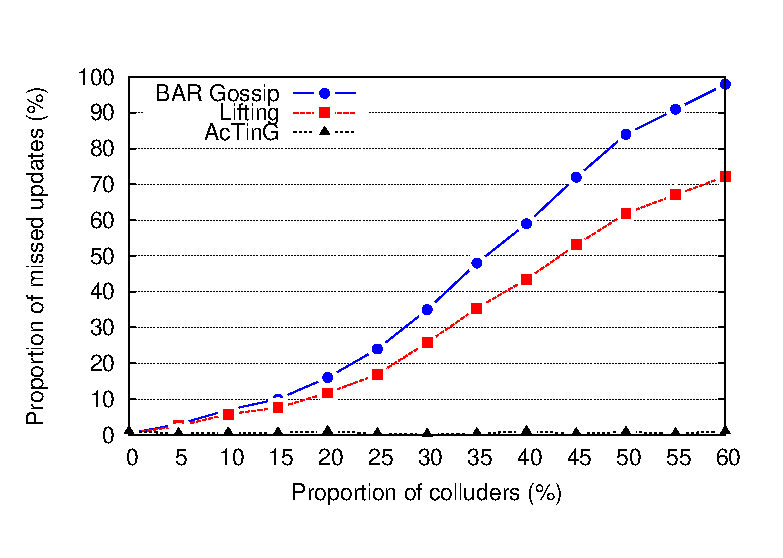
\includegraphics[width=.7\textwidth]{fig/delivery_rate_250}
      \end{figure}
      \vfill
      \begin{block}{}
        When 15\% of nodes collude, correct nodes miss 10\% of the content.
      \end{block}
   \endminipage
\end{frame}

\begin{frame}{Impact of collusions}{Scenario 2/2: Several coalitions}
%-------------------------------------------------------
   \minipage[c][0.7\textheight][s]{\textwidth}
      \begin{figure}
      \centering
      \includegraphics[width=.7\textwidth]{fig/delivery_rate_250_several_group}
      \end{figure}
      \vfill
      \begin{block}{}
        30\% of nodes collude. The size of colluding groups does not change the observation. Even groups of 2 nodes degrade performance noticeably.
      \end{block}
   \endminipage
\end{frame}

\subsection{Idea 1: Deterministic behavior}

\begin{frame}{Key ideas of AcTinG 1/3}{Deterministic behavior}
%-------------------------------------------------------
   \minipage[c][0.7\textheight][s]{\textwidth}
      It should be possible to predict how a node interacts with other nodes. 
      \begin{block}{}
      \begin{itemize}
        \item Nodes are synchronized, and time is structured as a sequence of rounds. 
        \item A PRNG guides associations between nodes.
        \item Sub-protocols are deterministic. 
      \end{itemize}
      \end{block}
      \begin{block}{Limitation}
      This is not enough as selfish nodes can choose not to initiate exchanges. 
      \end{block}
   \endminipage
\end{frame}

\subsection{Idea 2: Accountability}

\begin{frame}{Key ideas of AcTinG 2/3}{Accountability}
%-------------------------------------------------------
   \minipage[c][0.7\textheight][s]{\textwidth}
      It should be possible to check the behavior of nodes, and make them responsible for their declarations. 
      \begin{block}{}
      \begin{itemize}
        \item Session key pair consisting of a public and a private key, that is used to sign messages.
        \item Secure log, tamper-evident and append-only, to record the messages sent, or received. 
      \end{itemize}
      \end{block}
      \begin{block}{Limitation}
      This is not enough as nodes can hide the updates they receive from accomplices. To do that, they would maintain different log versions. 
      \end{block}
   \endminipage
\end{frame}

\subsection{Idea 3: Audits}

\begin{frame}{Key ideas of AcTinG 3/3}{Audits}
%-------------------------------------------------------
   \minipage[c][0.7\textheight][s]{\textwidth}
      It should be possible to compare the declarations of a node to detect errors, or equivocations. 
      \begin{block}{}
      Use \textbf{verifiable, random yet unpredictable audits}. 
      \begin{itemize}
        \item Verifiable: if a selfish node decides not to audit other nodes, it should be eventually discovered by correct nodes. 
        \item Random: the overhead due to audits is decreased
        \item Unpredictable: if a selfish node can predict whether or not it will be audited, then it would choose when to execute its deviations. 
      \end{itemize}
      \end{block}
      \begin{block}{Conclusion}
      Deviating from the protocol means taking a high, and unpredictable, risk of being detected. 
      \end{block}
   \endminipage
\end{frame}

\subsection{Audit and collusions in AcTinG}

\begin{frame}{Audit and collusions in AcTinG}{}
%-------------------------------------------------------
   \minipage[c][0.8\textheight][s]{\textwidth}
      \begin{center}
         \includegraphics[height=0.8\textheight]<1>{fig/Audit/1}
         \includegraphics[height=0.8\textheight]<2>{fig/Audit/2}
         \includegraphics[height=0.8\textheight]<3>{fig/Audit/3}
         \includegraphics[height=0.8\textheight]<4>{fig/Audit/4}
         \includegraphics[height=0.8\textheight]<5>{fig/Audit/5}
         \includegraphics[height=0.8\textheight]<6>{fig/Audit/6}
         \includegraphics[height=0.8\textheight]<7>{fig/Audit/7}         
         \includegraphics[height=0.8\textheight]<8>{fig/Audit/8}
         \includegraphics[height=0.8\textheight]<9>{fig/Audit/9}
         \includegraphics[height=0.8\textheight]<10>{fig/Audit/10}
         \includegraphics[height=0.8\textheight]<11>{fig/Audit/11}
         \includegraphics[height=0.8\textheight]<12>{fig/Audit/12}
         \includegraphics[height=0.8\textheight]<13>{fig/Audit/13}
         \includegraphics[height=0.8\textheight]<14>{fig/Audit/14}
         \includegraphics[height=0.8\textheight]<15>{fig/Audit/15}
      \end{center}
   \endminipage
\end{frame}

\subsection{AcTinG's properties}

\begin{frame}{AcTinG's properties}{}
%-------------------------------------------------------
   \minipage[c][0.7\textheight][s]{\textwidth} 
      \begin{block}{}
      AcTinG forces any node to:
      \begin{itemize}
        \item interact with other nodes
        \item receive the updates officially
        \item forward updates to its partners 
        \item audit its partners 
        \end{itemize}
      \end{block}
      
      \begin{block}{Remark}
      Nodes can still exchange updates off the record, but it is not interesting. They will be forced to receive them officially anyway. 
      \end{block}
      
   \endminipage
\end{frame}

\subsection{Performance evaluation}

\begin{frame}{Performance evaluation}{Probabilistic audit}
%-------------------------------------------------------
   \begin{block}{How efficient are audits?}
      \begin{itemize}
        \item Audits are triggered randomly, with a probability of 5\%
        \item When 10\% of the audience collude in a single group, any collective deviation is detected with a probability of 60\%.
        \item The only possible deviation brings a long term gain of only 3\%, and is eventually detected. 
        \end{itemize}
   \end{block}
\end{frame}

\begin{frame}{Performance evaluation}{Bandwidth consumption}
%-------------------------------------------------------
  \begin{center}
     \includegraphics[height=.6\textheight]{fig/uploadBandwidth.pdf}
  \end{center}
\end{frame}

%-------------------------------------------------------
\section{Problem 2: Privacy with Selfish Nodes}
%-------------------------------------------------------

\subsection{Problem presentation}

\begin{frame}{Privacy issues}{}
%-------------------------------------------------------
   \begin{itemize}
      \item Users are more and more aware that applications, or other persons, may collect data about them, and later study or leak this data. 
\vspace{5mm}
      \item They may be reluctant to use a gossip protocol where other users can learn information about them. AcTinG collects information in logs, and share these logs. 
\vspace{5mm}      
      \item One approach is to design applications that are not able to collect any private data due to encryptions. 
   \end{itemize}
\end{frame}

\begin{frame}{Problem 2}{Privacy in presence of selfish nodes}
%-------------------------------------------------------
% \minipage[c][0.7\textheight][s]{\textwidth}    
%    \begin{block}{}
      \textbf{Existing solutions against selfish nodes} in gossip are not privacy preserving:
         \begin{itemize}
            \item Symmetric exchanges and pseudorandomness: predictability of interactions
            \item Reputation-based: logs, and verification procedures
            \item Accountability: public secure logs
            \item Anonymous communication systems: too costly 
         \end{itemize}
%    \end{block}
 
  \begin{block}{Problem 2: Privacy in presence of selfish nodes}
     \textbf{Current protocols leak information} about users, which may drive them away, or \textbf{are too costly}.
  \end{block}
 
% \endminipage
\end{frame}

\subsection{Assumptions}
\begin{frame}{Assumptions}{} 
   \begin{block}{}
   We assume that
   \begin{itemize}
   \item All nodes are selfish
   \item A selfish node avoids to provide evidence that it is faulty to a node that it does not trust
   \item \sout{They may collude to increase their benefit, or avoid being detected}
   \item All nodes are curious
   \item An attacker may control a given proportion of nodes, and try to obtain information
   \end{itemize}
   \end{block}
\end{frame}

\subsection{Contribution details}
\begin{frame}{Contributions}{Accountability and privacy}
%-------------------------------------------------------
      \begin{enumerate}
        \item New privacy-preserving verification that a node forwarded messages
        \item Proof of security using a cryptographic protocol verifier (ProVerif)
        \item Design of a new protocol resistant to selfish nodes and privacy-preserving: PAG
        \item Evaluation of a prototype
        \begin{itemize}
          \item Deployments on Grid5000 (Java)
          \item Omnet++ simulations (C++)
          \item Bandwidth and CPU consumptions
          \item Probabilities that information is obtained by an attacker
          \end{itemize}
      \end{enumerate}
\end{frame}

\subsection{Properties against selfishness}
\begin{frame}{Properties to enforce}{}
%-------------------------------------------------------
% \minipage[c][0.7\textheight][s]{\textwidth} 
   As we saw in Part 1, the following properties have to be enforced against selfish nodes:
     \begin{itemize}
        \item $\mathbf{R_1}$: Obligation to receive updates
        \item $\mathbf{R_2}$: Obligation to forward updates
        \item $\mathbf{R_3}$: Random associations
     \end{itemize}
%      \vfill
   \vspace{5mm}
   However, it is a challenge to do it while hiding the following information:
   \begin{itemize}
        \item $\mathbf{P_1}$: Contents nodes are interested in
        \item $\mathbf{P_2}$: Group of nodes interested in the same content
        \item $\mathbf{P_3}$: Details of all interactions
   \end{itemize}
   
% \endminipage
\end{frame}

\subsection{Idea 1: Global membership}
\begin{frame}{Key ideas of PAG 1/3}{Global membership}
%-------------------------------------------------------
\minipage[c][0.7\textheight][s]{\textwidth} 
  \begin{block}{Idea 1: Hiding the interests of nodes $\longrightarrow \mathbf{P_1}, \mathbf{P_2}$}
  Merge $k$ content dissemination sessions maintained using Fireflies.\\
  The successors of a node are determined using a pseudorandom number generator among the full membership.
  \end{block}
  
  \only<1> {
  \begin{center}
     \includegraphics[height=.4\textheight]{fig/PAG/multisessionsExchanges}
  \end{center}
  }
  
  \only<2> {
    \begin{block}{Limitation}
  Properties $\mathbf{R_1}$, $\mathbf{R_2}$ and $\mathbf{R_3}$ are not enforced: a node can be selfish.  
  \end{block}
  }
  
\endminipage
\end{frame}

\subsection{Idea 2: Monitoring infrastructure}
\begin{frame}{Key ideas of PAG 2/3}{Accountability through monitoring}
%-------------------------------------------------------
\minipage[c][0.7\textheight][s]{\textwidth} 
  \begin{block}{Idea 2: Using a monitoring infrastructure $\longrightarrow \mathbf{P_1}, \mathbf{P_2}, \mathbf{R_1}, \mathbf{R_2}, \mathbf{R_3} $}
  Each node is affected a set of monitors that check that it behaves correctly, and inform the monitors of its successors that they receive an update. 
  \end{block}
  \vfill
  \only<1> {
  \begin{center}
     \includegraphics[height=.4\textheight]{fig/PAG/AccountableGossip}
  \end{center}
  }
  
  \only<2> {
  \begin{center}
     \includegraphics[height=.4\textheight]{fig/PAG/firefliesMembership}
  \end{center}
  }
  
  \only<3> {
    \begin{block}{Limitation}
  Property $\mathbf{P_3}$ is not enforced. Monitors should not be able to understand the exchanges they check. 
  \end{block}
  }
\endminipage
\end{frame}

\subsection{Idea 3: Homomorphic encryption}
\begin{frame}{Key ideas of PAG 3/3}{Privacy of exchanges}
%-------------------------------------------------------
  \begin{block}{Idea 3: Homomorphic hash function $\longrightarrow \mathbf{P_1}, \mathbf{P_2}, \mathbf{P_3}, \mathbf{R_1}, \mathbf{R_2}, \mathbf{R_3} $}
  \begin{itemize}
  \item We use a hash function based on RSA, where $\{u\}_{(e,m)} = u^e mod\ m$
  \vspace{5mm}
  \item Homomorphic properties
  \begin{itemize}
  \item $\{u_1\}_{(e,m)} \cdot \{u_2\}_{(e,m)}  = \{u_1 \cdot u_2\}_{(e,m)}$ 
  \item $\left\{ \{u\}_{(e_1,m)} \right\}_{(e_2, m)} = \{u\}_{(e_1 \cdot e_2,m)}$
  \end{itemize}
  \vspace{5mm}
  \item The monitors use these properties to check that a node forwards what it receives, without learning the contents of the exchanges.
  \end{itemize}
  \end{block}
\end{frame}

\begin{frame}{Key ideas of PAG 3/3}{Privacy of exchanges}
%-------------------------------------------------------
\begin{center}
   \includegraphics[width=\textwidth]{fig/PAG/intuition}
\end{center}
\end{frame}

\subsection{Summary of PAG}
\begin{frame}{Summary of PAG}{}
%-------------------------------------------------------
\minipage[c][0.7\textheight][t]{\textwidth} 
  \begin{block}{The desired properties are enforced}
  \begin{itemize}
  \item $\mathbf{P_1}$ and $\mathbf{P_2}$: $k$ contents are distributed simultaneously
  \item $\mathbf{R_1}$, $\mathbf{R_2}$ and $\mathbf{R_3}$: each node has a set of monitors that check that the received updates are forwarded
  \item $\mathbf{P_3}$: Homomorphic encryptions. Nodes interested by different contents check each other, and do not understand the exchanges.
  \end{itemize}
  \end{block}
\endminipage
\end{frame}

\subsection{Performance evaluation}
\begin{frame}{Security guarantees}{}
%-------------------------------------------------------
   \begin{itemize}
      \item We consider a global and active opponent that may control nodes to break the privacy of the exchanges of other nodes.
      \item We proved PAG using a cryptographic protocol verifier (ProVerif)
      \item Controlling $f$ nodes may threaten property $\mathbf{P_3}$.
   \end{itemize} 
  
   \begin{center}
      \includegraphics[height=.55\textheight]{fig/PAG/probaPrivacy}
   \end{center}
\end{frame}

\begin{frame}{Bandwidth consumption}{}
%-------------------------------------------------------
   \begin{center}
      \includegraphics[height=.55\textheight]{fig/PAG/scalability}
   \end{center}
\end{frame}


%-------------------------------------------------------
\section{Conclusion and Future Works}
%-------------------------------------------------------

% \begin{frame}{Conclusion}{}
% %-------------------------------------------------------
% \begin{itemize}
% \item Tolerating faults in distributed systems now implies the use of monitoring, or cryptography. 
% \item Novel data structures, or mechanisms may extend the privacy of users to new domains. 
% \end{itemize}
% \end{frame}

\begin{frame}{Possible improvements}{}
%-------------------------------------------------------
\begin{itemize}
   \item Combine both AcTinG and PAG to deter collusions \textbf{and} protect the privacy of users.
   \item In PAG, nodes simultaneously receive $k$ contents. It would be interesting to decrease the overhead of the protocol: receive mostly the content of interest, and less the others.
\end{itemize}
\end{frame}


{\2
\begin{frame}[plain,noframenumbering]
  \finalpage{Thank you for your attention.\\ \Huge{Questions?}}
\end{frame}}

\end{document}